% -*-LaTeX-*-

% $Log: intro.tex,v $
% Revision 1.5  2007/11/25 02:46:08  stiber
% Revisions for Winter 2008, including updated roadmap and
% typographical conventions.
%
% Revision 1.4  2007/11/25 01:49:33  stiber
% Additional revisions for stand alone book for Spring 2007.
%
% Revision 1.3  2007/03/04 19:34:08  stiber
% Initial revision for stand-alone textbook.
%
% Revision 1.2  2004/03/29 19:46:22  stiber
% Updated for Spring 2004 and new textbook (DSP First).
%
% Revision 1.1  2004/02/19 00:20:54  stiber
% Initial revision
%

\chapter*{Preface}
\addcontentsline{toc}{chapter}{Preface}

\markboth{PREFACE}{}

As computers become ubiquitous, they become more and more embedded not
only in the devices we own and use but in our lives. As a result,
computers become embedded in the physical world, with their primary
purpose being to detect and analyze happenings in our world and to
produce responses that affect that world. As computing professionals,
we need to understand how computers can process information from the
physical world as \emph{digital signals}: multimedia (sound, images,
video) and other measurements (in medical instruments, cars, cell
phones, eyeglasses, etc). This is why we have chosen to coin the
phrase ``Signal Computing''.

Digital signals place great demands on processing power, network
bandwidth, storage capacity, I/O speed, and software design. As a
result, signal computing is a great laboratory for exercising the full
range of knowledge of computer science.

In this book, you will learn how digital signals are captured,
represented, processed, communicated, and stored in computers. The
specific topics we will cover include: physical properties of the
source information (such as sound or images), devices for information
capture (microphones, cameras), digitization, compression, digital
signal representation (JPEG, MPEG), digital signal processing (DSP),
and network communication.  By the end of this book, you should
understand the problems and solutions facing signal computing systems
development in the areas of user interfaces, information retrieval,
data structures and algorithms, and communications.

While there certainly may be many opportunities for you to work in
signal computing, the value of this study extends far beyond. Studying
signal computing and its underlying mathematics directly exercises key
computer science abilities in areas like abstraction and
algorithmics. You will see that this book interleaves mathematical
topics with applications and algorithms. At each step of the way, we
take a representation of digital signals or operations on them that you
are familiar with, reach a concept in which it is awkward or difficult
to use, and then develop an alternative representation that simplifies
matters. This is exactly what computing professionals do in their
careers --- identify that a problem at hand can be represented by some
abstraction with known properties that can be manipulated by
well-understood algorithms. We hope that the journey you take through
the mathematical abstractions here will not only give you an important
set of tools to use later on, but will also help exercise your
fundamental ability to move from one representation to another.

Beyond your own personal professional capabilities, we hope that this
book will also give you a better understanding of the design process
that electrical engineers go through when they design the details of
signal processing systems, such as filters. Even if you do not go on
to build software components that perform signal processing, there is
a good chance that you will work on large systems that have DSP
components. We believe that it will be invaluable for you to
understand the basics of how such DSP components work and what your
electrical engineering colleagues are working on.

\section*{Objectives}
\addcontentsline{toc}{section}{Objectives}

By the end of this book, you should know:

\begin{itemize}
\item What physical signals are like in the ``real'' world and how
  their properties affect how we perceive them.
\item How these signals are \emph{digitized} and the tradeoffs among
  sampling speed, levels of quantization, file size, etc.
\item How to perform simple signal filtering to remove noise,
  emphasize important features, etc.  You should be well-prepared to
  work with electrical engineers in the design of more advanced signal
  processing systems.
\item How to carry out simple time-series analysis techniques to
  analyze frequency and characterize unknown signals.
\item How multimedia file sizes can be reduced by compression, and the
  tradeoffs among compression, processing overhead, and media quality.
\end{itemize}

\section*{Prerequisites}
\addcontentsline{toc}{section}{Prerequisites}

This book covers much of the mathematical foundations for
understanding signals and signal processing; however, it is assumed
that you are familiar with topics such as complex numbers,
trigonometry, derivatives, vectors, the basic idea of integrals,
infinite series, and basic physics (mass, acceleration, force,
etc). Figure~\ref{fg:roadmap} shows these prerequisites in the context
of this book's chapters.

\begin{figure}
\vspace{2in}
\centerline{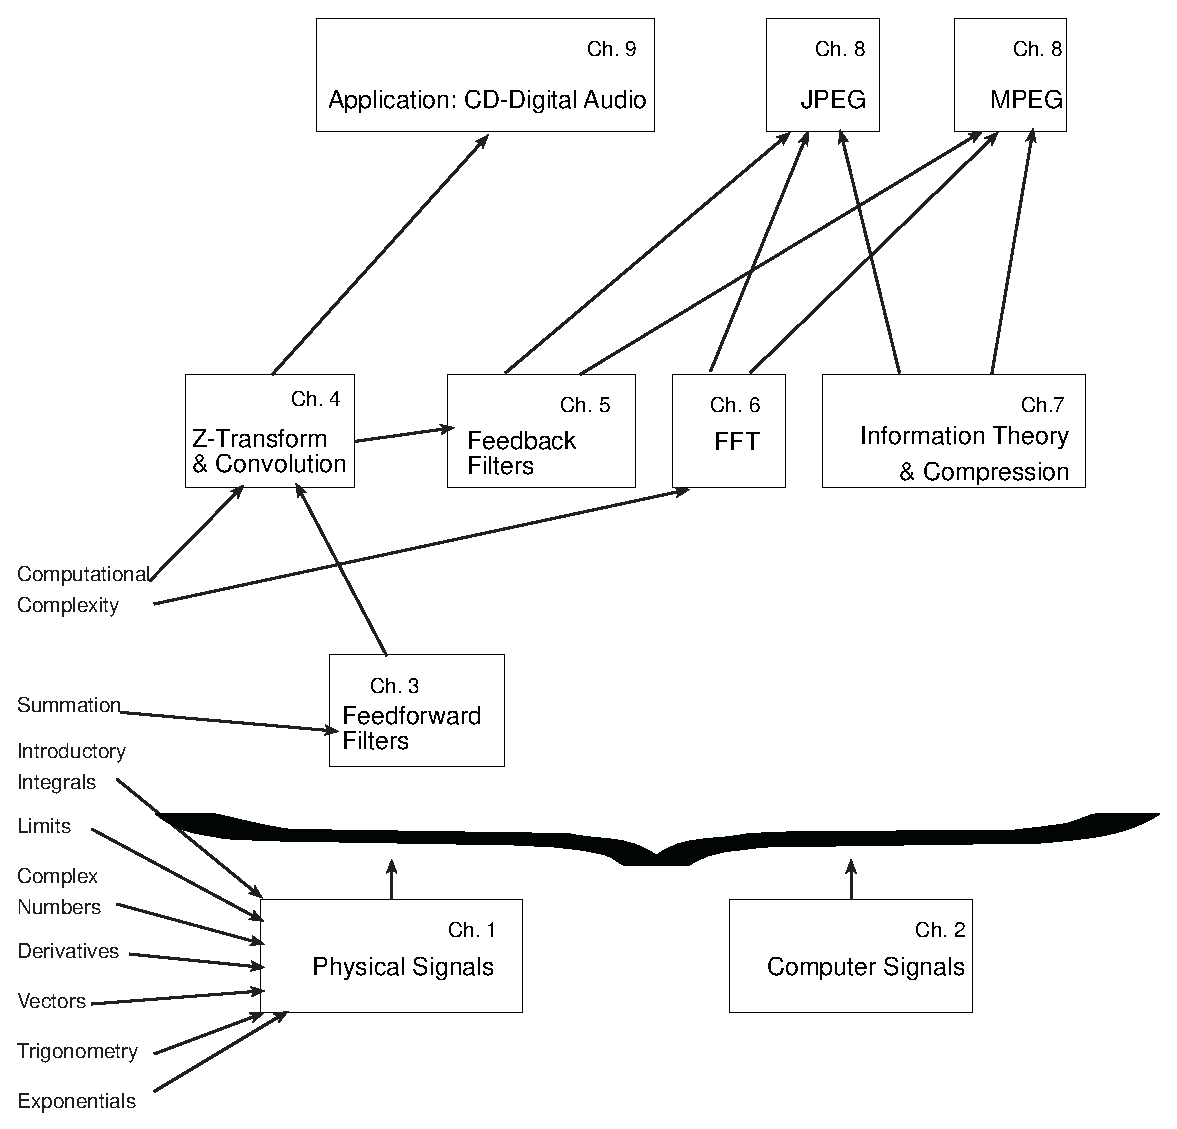
\includegraphics[width=0.9\textwidth]{roadmap}}
\caption[Course conceptual road map]{Course conceptual road
map and background knowledge.\label{fg:roadmap}}
\end{figure}

Figure~\ref{fg:roadmap} also outlines how each chapter's concepts are
used by subsequent ones and what the major themes are. You'll notice
that there's not much in the way of programming indicated. While there
\emph{is} an expectation that you understand the basics of
computational complexity and can understand, appreciate, and analyze
algorithms, this is \emph{not} a programming book. Instead, this is a
book that makes concrete many of the previously abstract mathematical
concepts that you are familiar with. It shows how these concepts
relate to \emph{real} applications that produce tangible changes on
digital signals --- it connects \emph{mathematics} to \emph{bits}.

As such, this book and the concepts within can be learned without any
explicit knowledge of low level programming in languages like C, C++,
or Java. Most of the exercises use an online, free tool known as Java
Digital Signal Processing (J-DSP) in order to put together block
diagrams using signal processing techniques.  Most of the problems
involving J-DSP require no background in any type of programming.

However, we also provide problems for students that have varying
levels of programming expertise (for example, you may have already
taken an algorithms or data structures class). If you have some
programming expertise, we provide problems that use simple Java
methods (or functions) in the J-DSP environment.  J-DSP provides a
coding template for you to use, in which you can fill in your own
simple manipulations of variables in the J-DSP environment using Java
and use block diagrams to manipulate signals further.  In this way,
you can focus on the implementation of different algorithms, not the
overhead involved in getting multimedia code working.  If you have
more experience in programming, we provide problems asking you to
write small programs in your choice of a ``lower level'' language
(such as C, C++, or Java).

\section*{About This Book}
\addcontentsline{toc}{section}{About This Book}

This book is divided into nine chapters. Chapters include self-test
exercises scattered throughout, so we suggest that you go through all
the material sequentially (or, at least, do the self-test exercises in
each section). Answers are provided at the back of the book. Each
chapter concludes with written or programming assignments and pointers
to additional readings.

\index{PDF} If you read the PDF version of this book, you will find
that it is extensively hyper-linked.  This includes links from
exercises to their answers, links to resources on the web, and links
from the table of contents, list of figures, index, etc. to their
respective locations.

Rather than distribute this book via a traditional publishing model,
costing you money and likely netting us very little, we have decided
to make this book freely available for both students and
faculty. Moreover, we have opened the source material for re-use,
updating, and expansion via a Creative Commons Attribution-ShareAlike
4.0 International License. This not only benefits you, it also
benefits us by getting our work into more people's hands.  You can
find the book's home page at
\url{http://faculty.washington.edu/stiber/pubs/Signal-Computing/},
including a pointer to its source material on GitHub. If you find any
errors, make any changes, or find this book useful in your course or
your life, please email us at \url{mailto:stiber@uw.edu}, or send us a
pull request.

\subsection*{Typographical Conventions}
\addcontentsline{toc}{section}{Typographical Conventions}

There are no real ``standards'' for much of the notation that is used
in digital signal processing; depending on which textbook you read,
you will encounter different typographical conventions. In this
textbook, we have chosen the following:
\begin{center}
\begin{tabular}{lp{5in}}
  $j$    & $\sqrt{-1}$ \\
  $t$    & continuous time; units typically seconds \\
  $x(t)$ & a real-valued function of continuous time (physical signal) \\
  $f$    & continuous frequency; units cycles/second or Hertz (Hz) \\
  $T$    & an interval of time; often $T=1/f$, meaning the period of a
           signal \\
  $f_0$  & a particular frequency; subscript may vary depending on use \\
  $\omega$ & continuous angular frequency; units radians/second \\
  $\omega_0$ & a particular angular frequency; subscript may vary
               depending on use \\
  $n$    & discrete time or sample number; dimensionless, but you can
           think of the units as being ``samples'' \\
  $x[n]$ & a function of discrete time; may be real-valued (sampled
           signal) or discrete valued (quantized/digital signal) \\
  $\hat{f}$ & discrete frequency; units cycles/sample \\
  $\hat{f}_0$  & a particular discrete frequency; subscript may vary
                 depending on use \\
  $\hat{\omega}$ & discrete angular frequency; units radians/sample \\
  $\hat{\omega}_0$ & a particular discrete angular frequency; subscript may vary
               depending on use \\
\end{tabular}
\end{center}

\section*{Further Reading}
\addcontentsline{toc}{section}{Further Reading}

An excellent introduction to digital signal processing that is
targeted at beginning electrical engineering students is \textit{DSP
  First: A Multimedia Approach}, by James H McClellan, Ronald
W. Schafer, and Mark A. Yoder (Prentice Hall, 1998).  It is important
to note that that book's target is the design of low-level signal
processing components (i.e., filters) and more generally linear,
time-invariant systems, rather than the role such components play in
overall software systems.
